\documentclass[10pt,a4paper]{article}

\usepackage{appendix}
\usepackage{graphicx}
\usepackage{parskip}
\usepackage{listings}
\usepackage{caption}
\usepackage{subcaption}
\usepackage{amsmath}
\usepackage{listings}
\usepackage{xcolor}
\usepackage[most]{tcolorbox}

%%%%%%%%%%%%%%%%%%%%%%%%%%%%%%%%%%%%%%%%%%%%%%%%%%%%%%%%%%%%%%%%%%%%%%%%%%%%%%%%%%%%%%%%%%%%%%%%%%%%%%%%%%
\definecolor{codegreen}{rgb}{0,0.6,0}
\definecolor{codegray}{rgb}{0.5,0.5,0.5}
\definecolor{codepurple}{rgb}{0.58,0,0.82}
\definecolor{backcolour}{rgb}{1,1,1}

\lstdefinestyle{mystyle}
{
    backgroundcolor=\color{backcolour},   
    commentstyle=\color{codegreen},
    keywordstyle=\color{magenta},
    numberstyle=\tiny\color{codegray},
    stringstyle=\color{codepurple},
    basicstyle=\ttfamily\footnotesize,
    breakatwhitespace=false,         
    breaklines=true,                 
    captionpos=b,                    
    keepspaces=true,                 
    numbers=left,                    
    numbersep=5pt,                  
    showspaces=false,                
    showstringspaces=false,
    showtabs=false,                  
    tabsize=2
}

\lstset{style=mystyle}
%%%%%%%%%%%%%%%%%%%%%%%%%%%%%%%%%%%%%%%%%%%%%%%%%%%%%%%%%%%%%%%%%%%%%%%%%%%%%%%%%%%%%%%%%%%%%%%%%%%%%%%%%%

\lstset{basicstyle=\ttfamily, breaklines = true, tabsize=2}
\graphicspath{ {./Images/} }
\setlength{\parskip}{1em}
\begin{document}
%%%%%%%%%%%%%%%%%%%%%%%%%%%%%%%%%%%%%%%%%%%%%%%%%%%%%%%%%%%%%%%%%%%%%%%%%%%%%%%%%%%%%%%%%%%%%%%%%%%%%%%%%%

\begin{titlepage}
	\centering
	{\scshape\LARGE Imperial College London \par}
	\vspace{1cm}
    {\scshape\Large ISA and Compilers: Year 2\par}
    \vspace{1.5cm}
	{\huge\bfseries Encoding and MIPS architecture \par}
	\vspace{2cm}
	{\Large\ Xin Wang }
	\vfill
	{\large \today\par}
\end{titlepage}

%%%%%%%%%%%%%%%%%%%%%%%%%%%%%%%%%%%%%%%%%%%%%%%%%%%%%%%%%%%%%%%%%%%%%%%%%%%%%%%%%%%%%%%%%%%%%%%%%%%%%%%%%%

\begin{abstract}
    In computer science, an instruction set architecture (ISA) is an abstract model of a computer.
    It defines the supported data types, the registers, the hardware support for managing main
    memory, and the input/output model of a family of implementations of the ISA. Most importantly,
    it specifies the behavior of machine code running on implementations of that ISA.

    MIPS (Microprocessor without Interlocked Pipelined Stages) is a reduced instruction set computer
    (RISC) ISA developed by MIPS Technologies. Often studied in university as later architectures
    are influenced by the ISC architecture used in MIPS.
\end{abstract}

%%%%%%%%%%%%%%%%%%%%%%%%%%%%%%%%%%%%%%%%%%%%%%%%%%%%%%%%%%%%%%%%%%%%%%%%%%%%%%%%%%%%%%%%%%%%%%%%%%%%%%%%%%

\tableofcontents
\pagebreak

%%%%%%%%%%%%%%%%%%%%%%%%%%%%%%%%%%%%%%%%%%%%%%%%%%%%%%%%%%%%%%%%%%%%%%%%%%%%%%%%%%%%%%%%%%%%%%%%%%%%%%%%%%
\section{Introduction}

To command a computer’s hardware, \textbf{instructions} need to be issued i.e. words of a 
computer’s language. The vocabulary is called an \textbf{instruction set}.

\begin{tcolorbox}[breakable,colback=white]
\textbf{Instruction set}: The vocabulary of commands understood by a given architecture.
\end{tcolorbox}

The Instruction Set Architecture (ISA) is the part of the processor that is visible to the
programmer or compiler writer. The ISA serves as the boundary between software and hardware. It
translates the high-level languages into machine code that is compatible with the hardware.

\begin{figure} [h!]
    \centering
    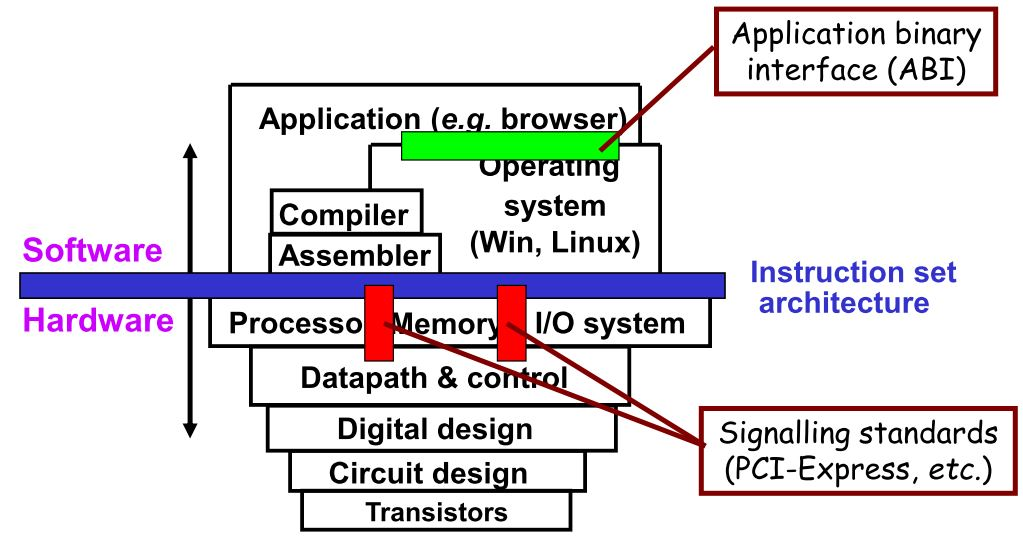
\includegraphics[scale=0.3]{ISA layers.JPG}
\end{figure}

In practice, computer hardware languages are quite similar. This is why MIPS architecture is studied as it
can easily be applied to the other types of architectures. MIPS are preferred over ARM as there are
simply much more academic source material for MIPS than there are for ARM. 

The similarity of instruction sets occurs because of two reasons:
\begin{itemize}
    \item All computers are constructed from hardware technologies based on similar fundamental
    principles.
    \item There are few basic operations that all computers must provide e.g. LDA and JMP.
\end{itemize} 
Computer designers have a common goal: Find a language that is: 
    \begin{itemize}
        \item Easy to use to implement the hardware.
        \item Maximising the performance.
        \item Minimising the cost to implement and the energy used.
    \end{itemize} 

By learning how to represent instructions as a compiler does, it includes an important discovery of
computing: the \textbf{stored-program concept}.
\begin{tcolorbox}[breakable,colback=white]
\textbf{Stored-program concept}: The idea that instructions and data of many types can be stored in
memory as numbers, leading to the concept of \textbf{stored-program computer}.
\end{tcolorbox}

%%%%%%%%%%%%%%%%%%%%%%%%%%%%%%%%%%%%%%%%%%%%%%%%%%%%%%%%%%%%%%%%%%%%%%%%%%%%%%%%%%%%%%%%%%%%%%%%%%%%%%%%%%
\section{Operations of the computer hardware}

Computer instructions are composed of the following: \textbf{Opcode} $+$ \textbf{Operand}.

Every computer must be able to perform fundamental arithmetic operations thus it is a good starting
point to understand a particular architecture.

In regards to basic addition, the MIPS assembly language notation:
\begin{lstlisting}[numbers=none]
    add a, b, c
\end{lstlisting}
instructs a computer to do the following:
\begin{enumerate}
    \item add the two variables \texttt{b} and \texttt{c}
    \item put the sum in \texttt{a}
\end{enumerate}
This notation is very rigid in that each MIPS arithmetic instruction performs only one operation and
\textbf{must always have exactly three variables}. Requiring every instruction to have exactly three
operands simplifies design because hardware for a variable number of operands is more complicated
than hardware for a fixed number of operands. This illustrates the first of three underlying
\textbf{principles of hardware design}:
\begin{tcolorbox}[breakable,colback=white]
\textbf{Hardware design principle 1}: Simplicity favors regularity.
\end{tcolorbox}

\textbf{Example 1}: This segment of a C program contains the five variables \texttt{a}, \texttt{b},
\texttt{c}, \texttt{d}, and \texttt{e}:
\begin{lstlisting}[numbers=none]
    a = b + c;
    d = a - e;
\end{lstlisting}
Translate from C to MIPS assembly language instructions like a compiler:
\begin{lstlisting}[numbers=none]
    add a, b, c
    sub d, a, e
\end{lstlisting}

%%%%%%%%%%%%%%%%%%%%%%%%%%%%%%%%%%%%%%%%%%%%%%%%%%%%%%%%%%%%%%%%%%%%%%%%%%%%%%%%%%%%%%%%%%%%%%%%%%%%%%%%%%
\section{Operands of computer hardware}

\begin{tcolorbox}[breakable,colback=white]
\textbf{Operand}: The part of a computer instruction which specifies what data is to be manipulated or operated on, while at the same time representing the data itself.
\end{tcolorbox}

Unlike high-level languages, the operands of arithmetic instructions are restricted; the operands
must be from a limited number of \textbf{registers} i.e. special locations built directly into the
hardware.

\begin{tcolorbox}[breakable,colback=white]
\textbf{Registers}: A temporary storage area built into the hardware, can be seen as the building
blocks of the computer.
\end{tcolorbox}

The standard size of a register in the MIPS architecture is \textbf{32 bits}, often grouped together as a
\textbf{word}. 
\begin{tcolorbox}[breakable,colback=white]
\textbf{Word}:  The natural unit of access in a computer, usually a group of 32 bits that
corresponds to the size of a register in the MIPS architecture.
\end{tcolorbox}

As there are a limited number of registers, usually 32 on current computers like MIPS, the three
operands of MIPS must each be chosen from one of the \textbf{32 32-bit registers}. 

The reason for the limit of 32 registers of each 32-bit is because a very large number of registers
may increase the clock cycle time simply with electronic signals taking longer to travel further.
This is the second design principle of hardware technology:
\begin{tcolorbox}[breakable,colback=white]
    \textbf{Hardware design principle 2}: Smaller is faster.
\end{tcolorbox}

The MIPS convention to represent a register is to \textbf{use two-character names following a dollar
sign} e.g. \texttt{\$s0}, \texttt{\$s1}, \dots, \texttt{\$s31}.

\textbf{Example 1}: It is the compiler’s job to associate program variables with registers. Given
the assignment statement:
\begin{lstlisting}[numbers=none]
    f = (g + h) - (i + j);
\end{lstlisting}
The variables \texttt{f}, \texttt{g}, \texttt{h}, \texttt{i}, and \texttt{j} are assigned to the
registers \texttt{\$s0}, \texttt{\$s1}, \texttt{\$s2}, \texttt{\$s3}, and \texttt{\$s4}
respectively. What is the compiled MIPS code?

Note that temporary registers \texttt{\$t0} and \texttt{\$t1} are used.
\begin{lstlisting}[numbers=none]
    add $t0,$s1,$s2 # register $t0 contains g + h
    add $t1,$s3,$s4 # register $t1 contains i + j
    sub $s0,$t0,$t1 # f gets $t0 - $t1
\end{lstlisting}

%%%%%%%%%%%%%%%%%%%%%%%%%%%%%%%%%%%%%%%%%%%%%%%%%%%%%%%%%%%%%%%%%%%%%%%%%%%%%%%%%%%%%%%%%%%%%%%%%%%%%%%%%%
\subsection{Memory operands}

Programming languages uses simple variables that contain single data elements to build more complex
data structures e.g. arrays. These complex data structures can contain many more data elements 
than registers can support.

The processor can keep only a small amount of data in registers but the computer memory can contain
much more data elements. Hence, complex data structures are kept in memory. MIPS includes \textbf{data
transfer instructions} that transfer data between memory and registers by supplying the memory
address to be accessed. Memory is just a large, single-dimensional array, with the address acting as the 
index to that array, starting at 0.

A MIPS data transfer instruction only reads one operand or writes one operand, without operating on
it. The data transfer instruction is called \textbf{load}. MIPS uses \texttt{lw} for \textit{loading
word} and format of the load instruction is:
\begin{enumerate}
    \item Name of the operation.
    \item The register to be loaded.
    \item A constant and register which the sum forms the memory address.
\end{enumerate} 

Because the compiler allocates data structures like arrays and structures to locations in memory, the compiler can then place the proper starting address into the data transfer instructions.

\textbf{Example 1}: Assuming that \texttt{A} is an array of $100$ words and that the compiler has
associated the variables \texttt{g} and \texttt{h} with the registers \texttt{\$s1} and
\texttt{\$s2} as before. Also assume that the starting address or base address of the array is in
\texttt{\$s3}. Compile this C assignment statement:
\begin{lstlisting}[numbers=none]
    g = h + A[8];
\end{lstlisting}
\begin{enumerate}
    \item Transfer A[8] to a register. The address of this array element is the sum of the base of
    the array A, found in register \texttt{\$s3}, plus the number to select element 8.
    \begin{lstlisting}[numbers=none]
        lw $t0, 8($s3) # $t0 gets A[8]
    \end{lstlisting}
    \item  Add content of \texttt{\$s2} to \texttt{\$t0} and put the sum in the register corresponding to \texttt{\$s1}.
    \begin{lstlisting}[numbers=none]
        add $s1,$s2,$t0 # g = h + A[8]
    \end{lstlisting} 
\end{enumerate}

Due to the fundamental nature of programs, 8-bit bytes are useful and virtually all architectures
address individual bytes. Therefore, the address of a word would match one of the address the 4
bytes within the word and addresses of sequential words would differ by 4. 
\begin{figure} [h!]
    \centering
    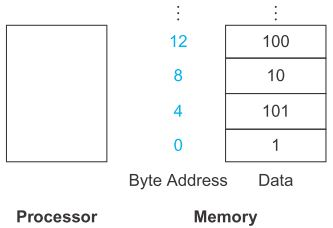
\includegraphics[scale=0.6]{4 bytes.JPG}
\end{figure}
In MIPS, words must start at addresses that are multiples of 4. This common architecture restriction
is known as an \textbf{alignment restriction}.
\begin{tcolorbox}[breakable,colback=white]
\textbf{Alignment restriction}: A requirement that data be aligned in memory on natural boundaries.
\end{tcolorbox}

The instruction complementary to load is traditionally called \textbf{store}. It copies data from a
register to memory and the format of a store is similar to that of a load: 
\begin{enumerate}
    \item The name of the operation: \texttt{sw}
    \item The register to be stored
    \item Offset to select the array element and the base register
\end{enumerate}

Registers take less time to access and have higher throughput than memory, making data in registers
both faster to access and simpler to use. Accessing registers also uses less energy than accessing
memory. It is these reasons that to achieve highest performance and conserve energy, an instruction set architecture must have a sufficient number of registers, and compilers must use registers efficiently.

%%%%%%%%%%%%%%%%%%%%%%%%%%%%%%%%%%%%%%%%%%%%%%%%%%%%%%%%%%%%%%%%%%%%%%%%%%%%%%%%%%%%%%%%%%%%%%%%%%%%%%%%%%
\subsection{Constant and immediate operands}

Many times a program will use a constant in an operation, many MIPS arithmetic instructions have a
constant as an operand. By including constants inside arithmetic instructions, operations are much
faster and use less energy than constants loaded from memory.

MIPS uses the add immediate \texttt{addi} instruction:
\begin{lstlisting}[numbers=none]
    addi $s3,$s3,4 # $s3 = $s3 + 4
\end{lstlisting}

Since MIPS supports negative constants, there is no need for subtract immediate in MIPS.

The \textbf{constant zero} has another role which is to simplify the instruction set by offering
useful variations. MIPS dedicates a register \texttt{\$zero} to be hard-wired to the value zero.
Using frequency to justify the inclusions of constants is another example of the great idea of
making the \textbf{common case fast}.

\pagebreak
%%%%%%%%%%%%%%%%%%%%%%%%%%%%%%%%%%%%%%%%%%%%%%%%%%%%%%%%%%%%%%%%%%%%%%%%%%%%%%%%%%%%%%%%%%%%%%%%%%%%%%%%%%
\section{Signed and unsigned numbers}

Numbers are kept in computer hardware as base 2 numbers. 
\begin{tcolorbox}[breakable,colback=white]
\textbf{Least significant bit}: The rightmost bit in a MIPS word.
\\
\\
\textbf{Most significant bit}: The left most bit in a MIPS word.
\end{tcolorbox}

\begin{figure} [h!]
    \centering
    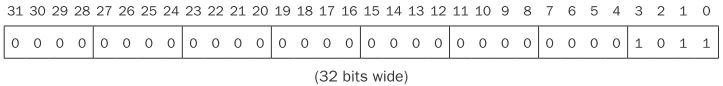
\includegraphics[scale=0.7]{32 bit MIPS}
\end{figure}
The MIPS word is 32 bits long, so can represent $2^{32}$ different 32-bit patterns. 

Hardware can be designed to add, subtract, multiply, and divide these binary bit patterns. If the
number that is the proper result of such operations cannot be represented by these rightmost
hardware bits, \textbf{overflow} has occurred. 

Computer programs calculate both positive and negative numbers, so a system to distinguishes the
positive from the negative is needed:
\begin{enumerate}
    \item \textbf{Sign and magnitude}: Simplest system but adders for sign and magnitude will need
    an extra step to set the sign because it is not known in advance what the proper sign will be.
    Also, a separate sign bit means that sign and magnitude has both a positive and a negative 
    zero, which can lead to problems.
    \item \textbf{Two’s complement}: Leading $0$s mean positive, and leading $1$s mean negative. It
    has the advantage that all negative numbers have a $1$ in the most significant bit i.e. the sign
    bit. Hardware needs to test only the sign bit to see if a number is positive or negative.
\end{enumerate}

Refer to Year 1 resources for revision on two's complement.

%%%%%%%%%%%%%%%%%%%%%%%%%%%%%%%%%%%%%%%%%%%%%%%%%%%%%%%%%%%%%%%%%%%%%%%%%%%%%%%%%%%%%%%%%%%%%%%%%%%%%%%%%%
\section{Representing Instructions in the Computer}

Instructions are kept in the computer as binary and \textbf{can be represented as numbers}. Each individual
piece of an instruction can be considered as an individual number, and placing these numbers side by
side forms the entire instruction.

There is a convention to mapping register names into a numbered format since registers are referred
to in instructions and instructions are numbers as mentioned earlier. This is covered in this
chapter.
\pagebreak
The following shows the real MIPS language version of the instruction represented symbolically, as a
decimal and binary.
\begin{lstlisting}[numbers=none]
    add $t0,$s1,$s2
\end{lstlisting}
\begin{figure} [h!]
    \centering
    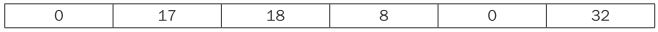
\includegraphics[scale=0.7]{Decimal example.JPG}
    \caption{Decimal format of the instruction}
\end{figure}
\begin{figure} [h!]
    \centering
    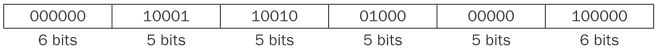
\includegraphics[scale=0.7]{Binary example.JPG}
    \caption{Binary format of the instruction}
\end{figure}

Each of these segments of an instruction is called a \textbf{field}.
\begin{itemize}
    \item  First $(0)$ and last $(32)$ field: Indicate to MIPS computer that this instruction performs addition.
    \item  Second $(17)$ field: Number of the register that is the \textbf{first source operand} of
    the addition operation i.e. $17 = \$s1$
    \item Third $(18)$ field: The other source operand for the addition i.e. $18 = \$s2$
    \item Fourth $8$ field: The number of the register that is to receive the sum i.e. $8 = \$t0$
    \item Fifth $0$ field: Usually deals with shift instructions, unused in this instruction so set to $0$.
\end{itemize}

Notice that all MIPS instruction takes exactly 32 bits, this is in keeping with the design principle
that simplicity favors regularity. This layout of the instruction is called the \textbf{instruction
format}.
\begin{tcolorbox}[breakable,colback=white]
\textbf{Instruction format}: A form of representation of an instruction composed of fields of binary numbers.
\end{tcolorbox}

To distinguish it from assembly language, the numeric version of instructions is called
\textbf{machine language} and a sequence of such instructions \textbf{machine code}.
\begin{tcolorbox}[breakable,colback=white]
\textbf{Machine language}: Binary representation used for communication within a computer system.
\end{tcolorbox}
Due to long binary numbers, using a higher base that can convert easily into binary, is much more
efficient. Since  all computer data sizes are multiples of 4, hexadecimal numbers are used.

\pagebreak
%%%%%%%%%%%%%%%%%%%%%%%%%%%%%%%%%%%%%%%%%%%%%%%%%%%%%%%%%%%%%%%%%%%%%%%%%%%%%%%%%%%%%%%%%%%%%%%%%%%%%%%%%%
\subsection{MIPS fields}

MIPS fields are given names:
\begin{figure} [h!]
    \centering
    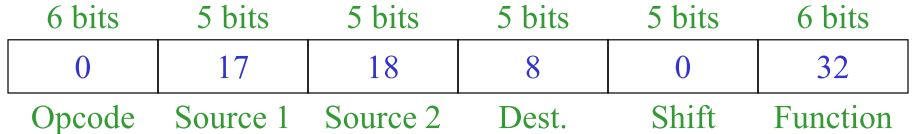
\includegraphics[scale=0.5]{MIPS field.JPG}
\end{figure}

A problem occurs when an instruction needs a longer field than those shown above. For example, with
the load word instruction must specify two registers and a constant. If the address were to use one
of the 5-bit fields in the format above, the constant used to select elements from arrays or data
structures would be limited to only $2^5$  or $32$. This 5-bit field is too small to be useful. This
leads to the fi nal hardware design principle: 
\begin{tcolorbox}[breakable,colback=white]
\textbf{Hardware design principle 3}: Good design demands good compromises. 
\end{tcolorbox}
The compromise chosen by the MIPS designers is to keep all instructions the same length and
requiring \textbf{different kinds of instruction formats} for different kinds of instructions.

Due to this compromise, MIPS has three types of instruction formats:
\begin{enumerate}
    \item \textbf{R-type} (Register): \par
    \begin{figure} [h!]
        \centering
        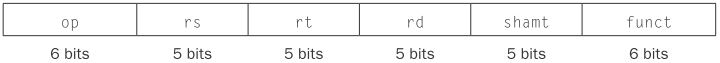
\includegraphics[scale=0.6]{R-type.JPG}
    \end{figure}
    Used by arithmetic instructions e.g. \texttt{add} and \texttt{sub}.
    \item \textbf{I-type} (Immediate): \par
    \begin{figure} [h!]
        \centering
        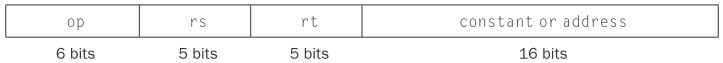
\includegraphics[scale=0.6]{I-type.JPG}
    \end{figure}
    Used by data transfer instructions e.g. \texttt{addi}, \texttt{lw} and \texttt{rw}. The 16-bit
    address means a load word instruction can load any word within a region of $\pm 2^{15}$ or $32,768$
    bytes of the address. Similarly, add immediate is limited to constants no larger than $\pm 2^{15}$. 
    \item \textbf{J-type} (Jump): \par
    \begin{figure} [h!]
        \centering
        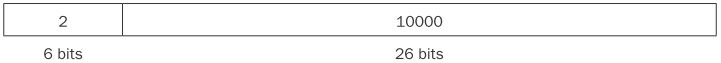
\includegraphics[scale=0.6]{J-type.JPG}
    \end{figure}
    The MIPS jump instructions have the simplest addressing. The J-type, which consists of $6$ bits for the operation field and the rest of the bits for the address field.
\end{enumerate}

Although multiple formats complicate the hardware, the complexity can be reduced by keeping some
parts of the formats similar.

%%%%%%%%%%%%%%%%%%%%%%%%%%%%%%%%%%%%%%%%%%%%%%%%%%%%%%%%%%%%%%%%%%%%%%%%%%%%%%%%%%%%%%%%%%%%%%%%%%%%%%%%%%
\section{Logical operators}

Although the first computers operated on full words, it was eventually clear that it was useful to
operate on \textbf{fields of bits within a word} or even on \textbf{individual bits}. These
instructions are called logical operations. \par
\begin{figure} [h!]
    \centering
    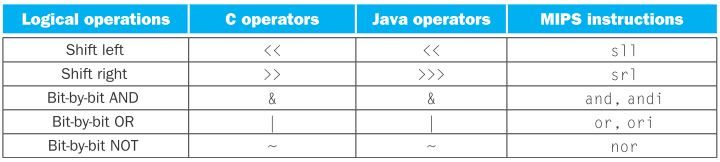
\includegraphics[scale=0.8]{Logical operator.JPG}
    \caption{Note:  MIPS implements NOT using a NOR with one operand being zero.}
\end{figure}
The first class of such operations is called \textbf{shifts} - shift left logical \texttt{sll} and
shift right logical \texttt{srl}. These instructions move all the bits in a word to the left or
right and filling the emptied bits with 0s. Shift left logical provides the equivalent of
multiplying by 2 per shift. 

For example, 
\begin{lstlisting}[numbers=none]
    sll  $t2,$s0,4  # reg $t2 = reg $s0 << 4 bits
\end{lstlisting}
where register
\texttt{\$s0} contained: 
\begin{lstlisting}[numbers=none]
    0000 0000 0000 0000 0000 0000 0000 1001 = 9
\end{lstlisting}
and the instruction to shift left by 4 was executed, the new value would be:
\begin{lstlisting}[numbers=none]
    0000 0000 0000 0000 0000 0000 1001 0000 = 144
\end{lstlisting}

Shift instructions are \textbf{R-type} instructions and uses the \textbf{shamt} field of the
R-format. Hence, the machine language version of the instruction above is:
\begin{figure} [h!]
    \centering
    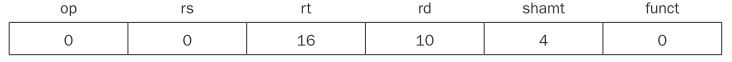
\includegraphics[scale=0.6]{Shift example.JPG}
\end{figure}

The second class are called \textbf{bit-by-bit operators} - AND and OR. AND is used to isolate
fields since it leaves a 1 in the result only if both bits of the operands are 1. Such a bit pattern
in conjunction with AND is called a \textbf{mask}, since the mask “conceals” some bits.

For example, 
\begin{lstlisting}[numbers=none]
    and $t0,$t1,$t2 # reg $t0 = reg $t1 & reg $t2
\end{lstlisting}
where register \texttt{\$t2} contains:
\begin{lstlisting}[numbers=none]
    0000 0000 0000 0000 0000 1101 1100 0000
\end{lstlisting}
and register \texttt{\$t1} contains:
\begin{lstlisting}[numbers=none]
    0000 0000 0000 0000 0011 1100 0000 0000
\end{lstlisting}
the value of register \texttt{\$t0} would be:
\begin{lstlisting}[numbers=none]
    0000 0000 0000 0000 0000 1100 0000 0000
\end{lstlisting}

The final logical operation is a \textbf{contrarian} - NOT takes one operand and places a $1$ in the
result if one operand bit is a $0$, and vice versa. In keeping with the three-operand format, the
designers of MIPS decided to use the instruction NOR instead of NOT. If one operand is zero, then it
is equivalent to NOT.

If the register \texttt{\$t1} is unchanged from the preceding example and register \texttt{\$t3} has
the value 0, the result of the MIPS instruction:
\begin{lstlisting}[numbers=none]
    nor $t0,$t1,$t3 # reg $t0 = NOT(reg $t1 | reg $t3)
\end{lstlisting}
the value in register \texttt{\$t0}:
\begin{lstlisting}[numbers=none]
    1111 1111 1111 1111 1100 0011 1111 1111
\end{lstlisting}

%%%%%%%%%%%%%%%%%%%%%%%%%%%%%%%%%%%%%%%%%%%%%%%%%%%%%%%%%%%%%%%%%%%%%%%%%%%%%%%%%%%%%%%%%%%%%%%%%%%%%%%%%%
\subsection{Instructions for Making Decisions}

The ability to make decisions is the distinguishing feature of a computer from a calculator. Based
on the input data and the values created during computation, different instructions execute.

MIPS assembly language includes two decision-making instructions, similar to an \textit{if}
statement with a \textit{go to}.
\begin{enumerate}
    \item \textbf{Branch if equal}: \texttt{beq register1, register2, L1}
    
    Go to the statement labeled \texttt{L1} if the value in \texttt{register1} \textbf{equals} the
    value in \texttt{register2}.
    
    \item \textbf{Branch if not equal}: \texttt{bne register1, register2, L1}
    
    Go to the statement labeled \texttt{L1} if the value in \texttt{register1} \textbf{does not equal} the value in \texttt{register2}.
\end{enumerate}

%%%%%%%%%%%%%%%%%%%%%%%%%%%%%%%%%%%%%%%%%%%%%%%%%%%%%%%%%%%%%%%%%%%%%%%%%%%%%%%%%%%%%%%%%%%%%%%%%%%%%%%%%%
\subsection{Loops}

Decisions are important both for choosing between two alternatives found in \textit{if} statements
and for iterating a computation found in loops.

There are three distinct types of loops in high level programming: \textbf{do/while}, \textbf{while}
and \textbf{for}. They are all functionally identical, any \textbf{for} loop can be turned into a
\textbf{while} loop with a bare minimum of effort.

Given a traditional loop in C:
\begin{lstlisting}[numbers=none]
    while (save[i] == k)
        i += 1;
\end{lstlisting}
where \texttt{i} and \texttt{k} correspond to registers \texttt{\$s3} and \texttt{\$s5} and the base of the 
array save is in \texttt{\$s6}. 

What is the MIPS assembly code corresponding to this C segment?
\begin{enumerate}
    \item Load \texttt{save[i]} into a temporary register \texttt{\$t1}. Before \texttt{i} is added to the base of
    array to form the address to load, multiply the index \texttt{i} by $4$ due to the byte
    addressing problem where each address has $4$ bits.
    \item To get the address of \texttt{save[i]}, add \texttt{\$t1} and the base of \texttt{save} in \texttt{\$s6}:
    \item Use that address to load \texttt{save[i]} into a temporary register:
    \item The next instruction performs the loop test, exiting if \texttt{save[i]} $\neq$ \texttt{k}:
    \item The next instruction adds 1 to \texttt{i}:
    \item The end of the loop branches back to the while test at the top of the loop. Add the Exit
    label after the loop.
    \begin{lstlisting}[numbers=none]
    Loop: sll $t1,$s3,2 # Temp reg $t1 = i * 4
        add $t1,$t1,$s6 # $t1 = address of save[i]
        lw $t0,0($t1) # Temp reg $t0 = save[i]
        bne $t0,$s5, Exit # Exit if save[i] != k
        addi $s3,$s3,1 # i = i + 1
        j     Loop # go to Loop
    Exit:
    \end{lstlisting}
\end{enumerate}

Sometimes it is useful to see if a variable is less than another variable. MIPS assembly language
has an instruction called \texttt{slt} (\textit{set on less than}) that compares two registers and sets a third register to:
\begin{itemize}
    \item $1$: if the first is less than the second
    \item $0$: otherwise
\end{itemize} 
\begin{lstlisting}[numbers=none]
    slt $t0, $s3, $s4   # $t0 = 1 if $s3 < $s4
\end{lstlisting}
There is an immediate version of the set on less than instruction. To test if register \texttt{\$s2} is less than the constant 
10:
\begin{lstlisting}[numbers=none]
    slti $t0,$s2,10     # $t0 = 1 if $s2 < 10
\end{lstlisting}

%%%%%%%%%%%%%%%%%%%%%%%%%%%%%%%%%%%%%%%%%%%%%%%%%%%%%%%%%%%%%%%%%%%%%%%%%%%%%%%%%%%%%%%%%%%%%%%%%%%%%%%%%%
\section{The processor}




%%%%%%%%%%%%%%%%%%%%%%%%%%%%%%%%%%%%%%%%%%%%%%%%%%%%%%%%%%%%%%%%%%%%%%%%%%%%%%%%%%%%%%%%%%%%%%%%%%%%%%%%%%
\end{document}